
\documentclass{article}
\usepackage{hyperref}
\usepackage{amsmath}
\usepackage{amssymb}
\usepackage{mathtools}
\usepackage{draftwatermark}


\SetWatermarkText{DRAFT}
\SetWatermarkScale{6}
\SetWatermarkLightness{0.95}

\title{A Consideration of Inflatable Circles}

\author{Robert L. Read
  \thanks{read.robert@gmail.com}
  email: \href{mailto:read.robert@gmail.com}{read.robert@gmail.com}\\
Megan Cadena
  \thanks{megancad@gmail.com}
  email: \href{mailto:megancad@gmail.com}{megancad@gmail.com}
  }


\begin{document}

\maketitle

\section{Introduction}
This is a study of the basic math of inflatable spheres as a tool for soft robotics.
We begin with a study in two dimension to simplify the problem.
Our final goal is to analyze three dimensional soft robots composed of inflatable
spheres.

\begin{figure}
     \centering
     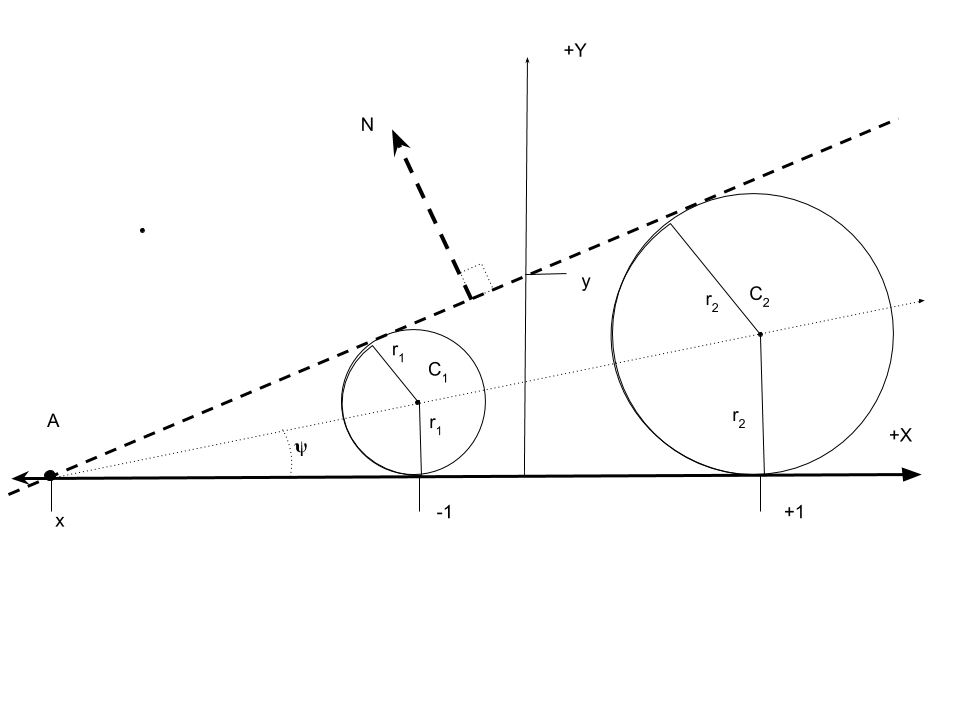
\includegraphics[width=0.80\textwidth]{figures/FixedAxisCircles.png}
     \caption{Problem I: Fixed Circles Centers}
  \label{fig:fixed}
\end{figure}

\section{Problem I: Circles in Fixed Postions}

A very simplified version of the problem is to imagine that a two-dimensional
plane.  Instead of spheres, we will assume we have circles of changable radius.
This is in fact realistic of a soft robot constrained to a plane.




Eventually we hope to have circles pressing against each other, or tangent
or ``kissing''. However, the problem is a bit simpler if we assume we have
two circles, each of which is constrained to have its center on the a vertical
line (see Figure \ref{fig:fixed}.)  We place the circle $C_1$ with radius $r_1$ on the $x = -1$ line, and
assume that it rests on a shelf or plane on the $x$-axis.
Assume the $C_2$ circle whose radius if $r_2$ is on the $x = 1$ line.

Let $A$ the intersection of the tangent line supported
by the inflatable circles with the $x$-axis. Call the distance of $A$
on the $x$-axis $x$. Let $\psi$ be the angle formed by the
circle centers with the $x$ axis (measured counterclockwise).

If the radii are less than $1$ so that no issues of intersection
of the circles arise, we have:

\begin{align}
  \tan{\psi} &= \frac{r_1}{x-1} = \frac{r_2}{x+1}  \\
  r_2(x - 1) &= r_1(x+1) \\
  r_2x - r_2 &= r_1x + r_1 \\
  r_2x - r_1x &= r_1 + r_2 \\
  x(r_2 - r_1) &= r_1 + r_2 \\
  x &= \frac{r_1+r_2}{r_2 - r_1} \\
  \tan{\psi} &= \frac{r_1}{x - 1} \\
  \psi &= \arctan{\frac{r_1}{x - 1}} \\
  N &=  \begin{bmatrix} -\sin{\psi} \\ \cos{\psi}  \end{bmatrix} \\
\end{align}





\section{Problem II: Tangent Circles}


\begin{figure}
     \centering
     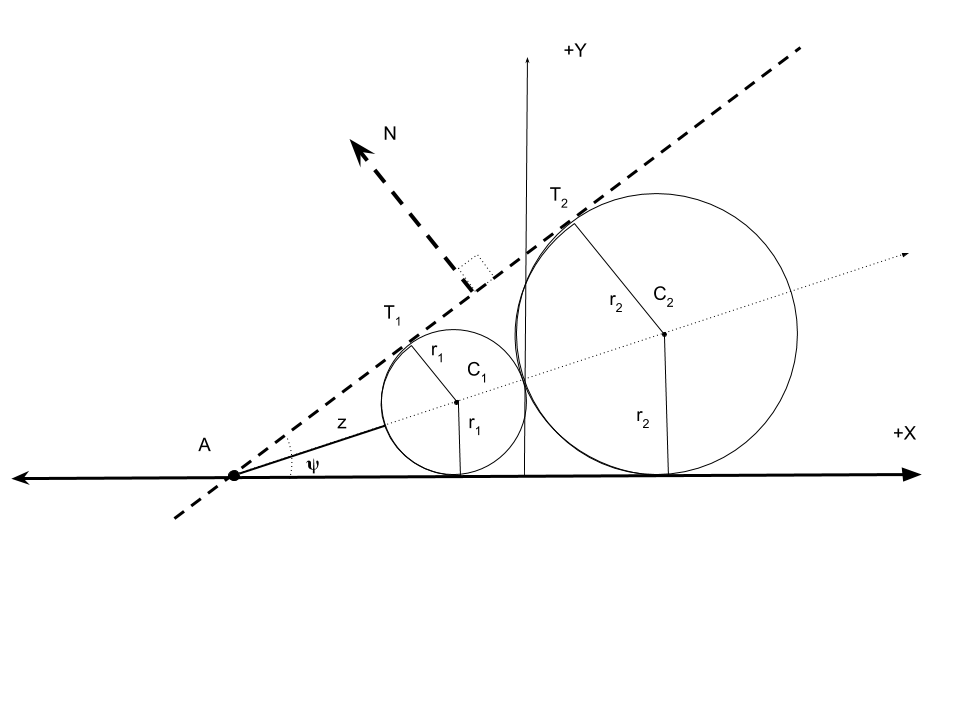
\includegraphics[width=0.80\textwidth]{figures/TangentCircles.png}
     \caption{Problem II: Tangent Circles}
  \label{fig:Tangent}
\end{figure}

\begin{align}
 %
\frac{r_2}{||(C2 - A)||} &= \frac{r_1}{||(C_1-A)||} \\
||C2 - A|| &= r_2+2r_1+z \\
||C1 - A|| &= r_1 + z \\
\frac{r_2}{r_2+2r_1+z} &= \frac{r_1}{r_1+z} \\
z &= -\frac{2 r_1^2}{r_1 - r_2} \text{ and } r_1 \neq r_2 \text{ and } r_1 r_2 (r_1 + r_2) \neq 0 \\
\sin{\psi} &= \frac{r_1}{z + r_1} \\
\theta &= \frac{2 \arcsin{r_1}}{z+r_1} \\
Nx &= -\sin{\pi/2 + \theta} \\
Ny &= -\cos{\pi/2 + \theta} \\
\end{align}
%
\end{document}


r2/||(C2 - A)|| = r1/||(C1-A)||
||C2 - A|| = r2+2*r1+z
||C1 - A|| = r1 + z
r2/(r2+2*r1+z) = r1/(r1+z)

z = -(2 r1^2)/(r1 - r2) and r1!=r2 and r1 r2 (r1 + r2)!=0

sin(psi) = r1/(z + r1)
Theta = 2 * arcsin(r1/(z+r1))
Nx = -sin(pi/2 + theta)
Ny = -cos(pi/2 + theta)


